\documentclass[tikz, rgb,dvipsnames]{standalone}
\usepackage{pgfplots}
\usepackage{xcolor}
\pgfplotsset{compat=newest}
\usetikzlibrary{calc,math}
\usetikzlibrary{shapes.misc}
\usetikzlibrary {arrows.meta}

\tikzset{>=latex}
\def\ColrGridLinesBackground{gray}
\def\ColrGridLinesFrame{black}
\def\Col{OliveGreen!15!white!75}

\def\ColA{red}
\def\ColB{red}
\def\ColC{red}
\def\W{5}
\def\H{5}

\newcommand{\Square}[1]{
\fill [color=#1]
(-\W, -\H) --
(-\W, \H) --
(\W, \H) --
( \W, -\H) -- cycle;


% frame around hexagon
\foreach \x in {-\W, ..., \W}
\foreach \y in {-\H,...,\H} {
    \draw [color=\ColrGridLinesFrame]
    (-\W, \y) -- (\W, \y)
    (\x, -\H) -- (\x, \H);
}
}

\newcommand{\Dot}[3] {
    \fill[color=#3] (2*#1, 2*#2) circle (0.075);
}

\newcommand{\Label}[4] {
    \node at (2*#1, 2*#2) [#3] {#4};
}

\begin{document}
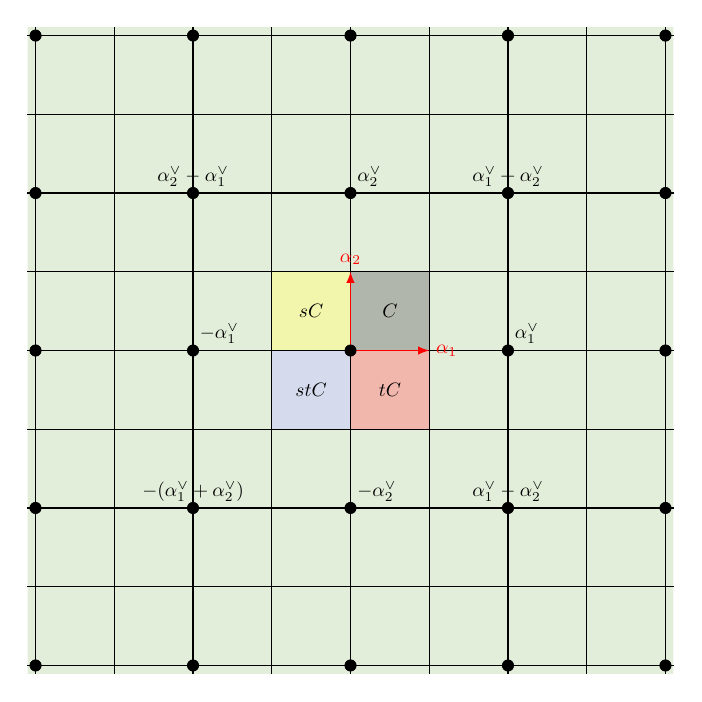
\begin{tikzpicture}[every node/.style={scale=0.7}]
    \clip (-\W+0.9, -\H+0.9) rectangle (\W-0.9, \H-0.9);

\Square{\Col}
\foreach \x in {-\W, ..., \W} {
\foreach \y in {-\H,...,\H} {
    \Dot{\x}{\y}{black}
}
}

\coordinate (O) at (0, 0);
\coordinate (A) at (1, 0);
\coordinate (B) at (1, 1);
\coordinate (C) at (0, 1);
\coordinate (D) at (-1, 1);
\coordinate (E) at (-1, 0);
\coordinate (F) at (-1, -1);
\coordinate (G) at (0, -1);
\coordinate (H) at (1, -1);

\fill[gray, opacity=0.5] (O) -- (A) -- (B) -- (C) -- cycle;
\fill[Yellow!50, opacity=0.5] (O) -- (C) -- (D) -- (E) -- cycle;
\fill[Blue!70!white!30!, opacity=0.5] (O) -- (E) -- (F) -- (G) -- cycle;
\fill[Red!50, opacity=0.5] (O) -- (G) -- (H) -- (A) -- cycle;

% background divisions
\draw [color=\ColrGridLinesFrame]
( -1, 0) -- (1, 0)
( 0, -1) -- (0, 1);
% frame around hexagon
\draw [color=\ColrGridLinesFrame]
(-1, -1) --
( 1, -1) --
( 1, 1) --
( -1,  1) -- cycle;


\draw[->, \ColA]
(0, 0) -- (0, 1) node[above] {$\alpha_2$};

\draw[->, \ColB]
(0, 0) -- (1, 0) node[below, right] {$\alpha_1$};


\foreach \x in {-\W,...,\W}
\foreach \y in {-\H,...,\H} {
    \Dot{\x}{\y}{black}
}


\coordinate (G) at (0.5, 0.5);
\node at (G) {$C$};

\coordinate (H) at (-0.5, 0.5);
\node at (H) {$sC$};

\coordinate (I) at (0.5, -0.5);
\node at (I) {$tC$};

\coordinate (J) at (-0.5, -0.5);
\node at (J) {$stC$};


\Label{1}{0}{above right}{$\alpha_1^\vee$}
\Label{0}{1}{above right}{$\alpha_2^\vee$}
\Label{1}{1}{above}{$\alpha_1^\vee+\alpha_2^\vee$}
\Label{-1}{0}{above right}{$-\alpha_1^\vee$}
\Label{-1}{-1}{above}{$-(\alpha_1^\vee+\alpha_2^\vee)$}
\Label{0}{-1}{above right}{$-\alpha_2^\vee$}
\Label{-1}{1}{above}{$\alpha_2^\vee-\alpha_1^\vee$}
\Label{1}{-1}{above}{$\alpha_1^\vee-\alpha_2^\vee$}
\end{tikzpicture}
\end{document}
